
\section{ByteNet}

\subsection{Validating Implementation}

Before using the model on the Europarl v7 dataset for solving the WMT Translation Task problem, the model is validated using some simpler datasets.

\subsubsection{Learning Synthetic Digits Problem}

The Synthetic Digits dataset is used for validating the generalization properties of the ByteNet implementation.

The internal dimensionality is set to 20, this is 20 units in the encoder and 40 units in the decoder, the latter is because the encoding is concatenated with the target embedding. It is unlikely that higher dimensionality is required, given that there are only 10 possible output characters. In fact, 20 might be much higher than necessary, but this may be a good thing in terms of validation as it provides an opportunity to ensure that the model doesn't overfit. Using a dimensionality of 20, the network has just counting the convolution and dense layers $73500$ weights. The training dataset contains only 128 observations, thus there is a huge potential for overfitting. The test dataset also contains 128 observations.

The ByteNet model is optimized using the Adam optimizer with a learning rate of 0.001 and a mini-batch size of 16 running on 1 GPU. Because the BLEU score is not meaningful for the Synthetic Digits problem, where no words exist in the target, the misclassification rate is calculated instead.

\begin{figure}[h]
    \centering
    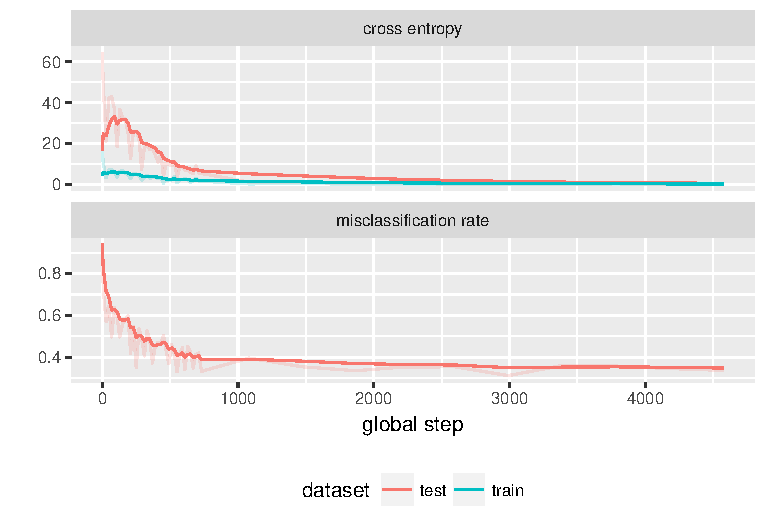
\includegraphics[scale=1]{bytenet/validation-synthetic-digits.pdf}
    \caption{Shows misclassification rate and the cross entropy loss. For comparison a the attention model has a misclassification rate of 0.51. The exponential moving average uses a forget factor of $0.1$.}
    \label{fig:result:bytenet:digits}
\end{figure}

\begin{table}[h]
\centering
\begin{tabular}{r|p{3.3cm} p{3.3cm} p{3.3cm}}
	obs. & source & target & prediction\\ \hline
  0 & one zero four & 104 & 104 \\
  1 & one five six & 156 & 150 \\
  2 & five five nine & 559 & 559 \\
  3 & one six & 16 & 68 \\
  4 & two three four & 234 & 235 \\
  5 & five three & 53 & 53
\end{tabular}
\caption{Source, target, and prediction on examples from the test dataset.}
\label{table:result:bytenet:digits}
\end{table}

Figure \ref{fig:result:bytenet:digits} shows reasonable convergence, only the test error shows jitter during training and there is very little overfitting if any. In the end, the ByteNet model completely learned the training dataset.

The jitter is likely not because of poor optimization, but rather because the errors are only calculated on a randomly sampled subset of the test dataset. For the different samples, the test error is thus different.

The lack of overfitting fits well with what the original ByteNet article also observed, in their translation model no regularization or early stopping was used, which is what one would typically use to prevent overfitting \cite{bytenet}.

In table \ref{table:result:bytenet:digits} the predictions are about what one would expect. For the most part, the translations are good, in particular in the beginning of the output sequence, while the later digit predictions show some error. This result is reasonable, as there is more data for the first two digits and because the input words have different lengths. The alignment between input and output characters becomes more uncertain as the read sequences get longer. Of cause, the model would ideally learn the word separation completely and understand that there is a direct relation between word and digit, but learning this relation is likely difficult given both the many parameters and the small dataset.

\clearpage
\subsubsection{Memorizing WMT NewsTest}

Sometimes a model works well when it has few weights and low dimensionality but breaks for higher dimensionality because of vanishing or exploding gradient issues. To validate that this is not an issue a good test is to see if the model can memorize a small dataset, but where the model complexity is kept high. For memorization one just expects the training loss to become very small, the test error is not important.

The WMT 2014 NewsTest dataset for German to English translation was used for training, this contains 3003 observations. The WMT 2015 NewsTest dataset was used for testing, this contains 1596 observations. The internal dimensionality is set to 400, (800 in the decoder because of concatenation).

The model ran 120 epochs over the training dataset, with a mini batch size of ${4 \cdot 16 = 64}$, running on 4 GPUs in parallel using synchronized updates with the Adam optimizer and a learning rate of 0.0003.

\begin{figure}[h]
    \centering
    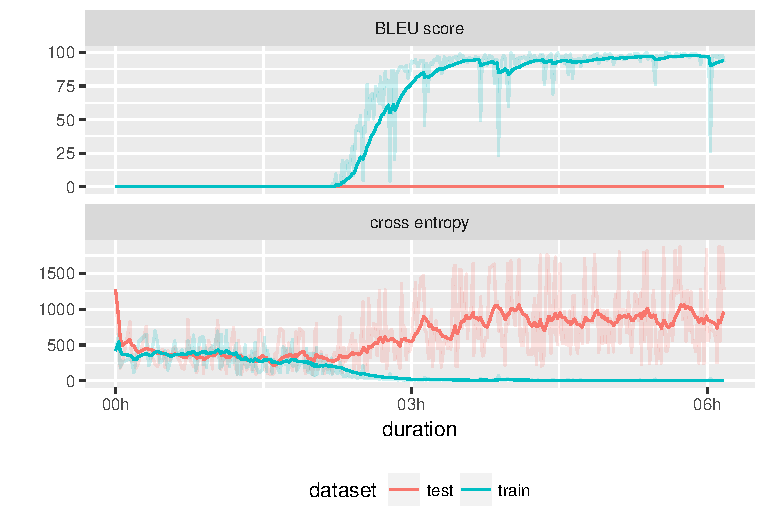
\includegraphics[scale=1]{bytenet/validation-memorize-wmt.pdf}
    \caption{Shows BLEU score and cross entropy loss for the German to English WMT NewsTest dataset. Both training and test measures are calculated on a randomly sampled mini-batch from each dataset. The exponential moving average uses a forget factor of $0.3$.}
    \label{fig:result:bytenet:wmt}
\end{figure}

\begin{table}[h]
\centering
\begin{tabular}{l|r|p{10cm}}
  0 & source & Polizei von Karratha verhaftet 20-Jährigen nach schneller Motorradjagd \\[0.1cm]
    & target & Karratha police arrest 20-year-old after high speed motorcycle chase \\[0.1cm]
    & translation & In must in the ugains of the with of Chanamby a leadn-Minor ald the ace the town of the construction of the compunity the government. \\[0.1cm]
    & BLEU & 0.00 \\[0.1cm] \hline
  1 & source & Das Motorrad wurde sichergestellt und für drei Monate beschlagnahmt. \\[0.1cm]
    & target & The motorcycle was seized and impounded for three months. \\[0.1cm]
    & translation & The New York works with smaries for twe to the come to cover earling scace us deliving the construction work. \\[0.1cm]
    & BLEU & 0.00
\end{tabular}
\caption{Source, target and prediction on the test dataset.}
\label{table:result:bytenet:wmt-test}
\end{table}

\begin{table}[h]
\centering
\begin{tabular}{l|r|p{10cm}}
  0 & source & Demgegenüber unterrichten australische Schulen durchschnittlich 143 Stunden jährlich und Schüler in Singapur erhalten 138 Stunden. \\[0.1cm]
    & target & By comparison, Australian schools provide an average of 143 hours a year and pupils do around 138 hours in Singapore. \\[0.1cm]
    & translation & By comparison, Australian schools provide an average of 143 hours a year and pupils do around 138 hours in Singapore. \\[0.1cm]
    & BLEU & 100.00 \\[0.1cm] \hline
  1 & source & Diese Umlage wird jedes Jahr im Oktober von den vier Betreibern der der großen Stromtrassen neu festgesetzt. \\[0.1cm]
    & target & This levy will be reset by the four operators of the large power grids, in October of each year. \\[0.1cm]
    & translation & This levy will be reset by the four operators of the lerge power grids, in October of each year. \\[0.1cm]
    & BLEU & 87.23
\end{tabular}
\caption{Source, target and prediction on the training dataset.}
\label{table:result:bytenet:wmt-train}
\end{table}

Ensuring that the optimization converges was the primary purpose of this experiment. Figure \ref{fig:result:bytenet:wmt} shows that the parameter optimization does like in the synthetic digits problem, appear to converge just fine. Initially, there is some jitter in the cross entropy training loss, but this subsides after awhile.

The jitter frequency is higher, in the beginning, this is just because TensorFlow samples values at fixed time intervals. Initially, there are some allocations and data transfers that causes the model to run slower, thus as a side effect TensorFlow samples more frequently in this period. 

As said the test loss is not very interesting, as there is isn't enough training data to expect the model to produce meaningful results. The cross entropy on the test dataset does also show an increase after the initial decrease, which indicates some overfitting. Again, this is to be expected given the small training dataset.

More interesting is the correlation between the training cross entropy and the training BLEU score. Initially, the cross entropy decreases a lot, but the BLEU score stays at 0. It is first when the cross entropy nears 0, that the BLEU score begins to improve. This observation is quite important as it indicates that cross entropy isn't a perfect loss measure for the translation problem. This is because the cross entropy can be quite low if it just gets the majority of the characters almost correct, but the position must be correct. The BLEU score, on the other hand, demands that the words matches exactly, but is looser regarding the position. For example, in table \ref{table:result:bytenet:wmt-train} the target is ``large'' but the prediction is ``lerge''. This is very close in terms of cross entropy but is completely wrong in terms of the BLEU score, since the words don't match. Nevertheless, the cross entropy loss is useful because its gradient in combination with softmax is easily computable, and the BLEU score does become very high in the end, even though the correlation between cross entropy and the BLEU score is weak.

The training BLEU score is actually extremely good, it shows almost a perfect translation. Typically translation models only show a BLEU score between 15 and 25 on a test set. This is not necessarily because the translation is wrong, but because there many different ways of translating a text correctly. The BLEU score does actually support multiple target sequences, but this is rarely provided in the test dataset because of the labor demands for creating multiple translations.

The only way the model can be this good is by primarily memorizing the output given the input. It is unlikely there is much understanding of the latent semantic meaning in the text. That being said, the predictions in table \ref{table:result:bytenet:wmt-test} shows that the model understands some grammar, such as which words comes before nouns. That being said, the second prediction example in table \ref{table:result:bytenet:wmt-test} contains a single quotation mark, which is not grammatically meaningful. 

Some of the above-mentioned issues could perhaps be improved by not using the target sequence in the decoder during training step. Instead, the predicted sequence could be used in the decoder input, just like in the inference model. This could solve issues like ``large'' becoming ''lerge''. The disadvantage of doing this is that training would be slower, as the decoder can't be parallelized over the sequence. Some research suggests that one should use a hybrid model, where the training loss is composed of both an assisted part and a non-assisted part, in the latter case the target sequence isn't used \cite{no-assist-train}.

Another observation is that the predicted sequences are in general a bit longer than the target sequences. This is likely because of how the sequence loss is constructed, this only measures the error where the target is explicitly known. Thus there is little penalty for predicting longer sequences than the target sequence. However, there is some penalty, because the predicted \texttt{<eos>} symbol should match the target \texttt{<eos>} symbol. More penalty could be added by padding the target sequence sufficiently with a special \texttt{<null>} symbol, and then also measure the error on that part of the sequence. However, this introduces an issue where the translation model can just predict ``\texttt{<null><null><null><null>...}'' and this will in terms of cross entropy be a good match since the majority of the sequence matches. This is an easily obtainable solution for the optimizer, it can thus be a local minimum that is difficult to escape.

\clearpage
\subsection{WMT Translation Task}

With the ByteNet model reasonably validated in terms of generalization on the synthetic digits problem, and convergence when memorizing the WMT NewsTest dataset, the ByteNet model is used on the Europarl v7 dataset for German to English translation.

\begin{figure}[h]
    \centering
    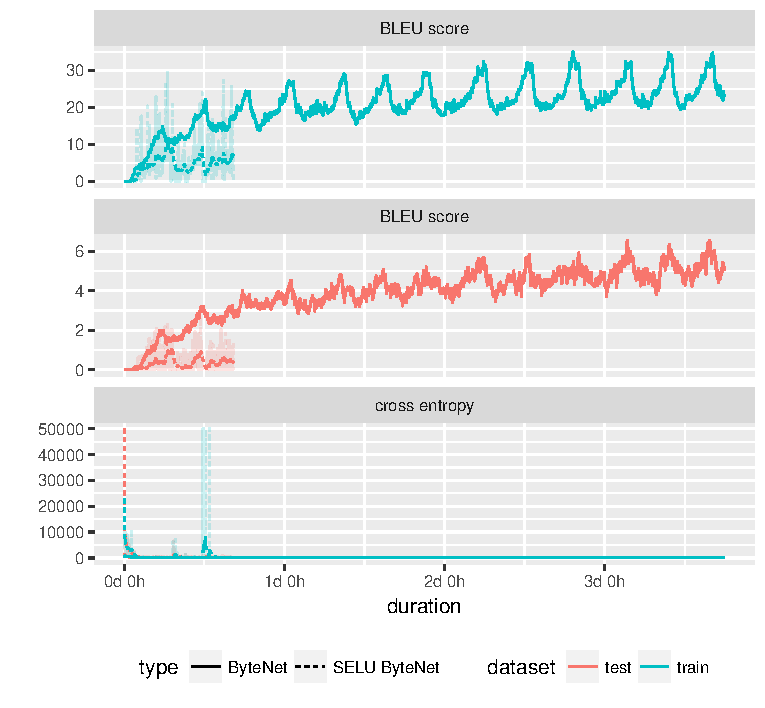
\includegraphics[scale=1]{bytenet/europarl.pdf}
    \caption{Shows BLEU score and cross entropy loss for ByteNet, trained on Europarl v7 and tested on WMT NewsTest 2015. Both training and test measures are calculated on a randomly sampled mini-batch from each dataset. The exponential smoothing uses a forget factor of $0.05$. The vertical lines separates each batch epoch.}
    \label{fig:result:bytenet:europarl}
\end{figure}

The ByteNet model has an internal dimensionality of 400, just like the model used for training on the WMT NewsTest dataset. The Adam optimizer with a learning rate of 0.0003 is used for training. This used a training mini-batch size of $4 \cdot 16 = 64$ observations and the model was trained on 4 GPUs in parallel with synchronized updates. The Europarl v7 dataset is used for training and the training ran 13 epochs over the Europarl v7 dataset. The WMT NewsTest 2015 dataset is used for testing, the continues testing was done on randomly sampled mini-batches with 128 observations each.

From figure \ref{fig:result:bytenet:europarl} it's seen that the BLEU score on the test dataset is approximately $5.5$. However, because that BLEU score is calculated on a random subset of the dataset it is not completely accurate. The actual BLEU score calculated on the entire WMT NewsTest dataset after training is $7.44$. The translations are shown in table \ref{table:result:bytenet:high-belu} and table \ref{table:result:bytenet:zero-belu}.

Figure \ref{fig:result:bytenet:europarl} also shows some oscillation that is correlated with the epochs. After further investigation it turns out that there are bad translations in the dataset, some examples can be seen in table \ref{table:result:bytenet:bad-translations}. Such observations would misdirect the optimization in each epoch and thus cause oscillation. However, even after removing all observations with either a source or target sequence less than 25 characters, the oscillation still exists. Given that the oscillation is correlated with the epochs, it is most likely the dataset that still contains poor observations. However, finding these among 2 million sentence pairs is rather difficult, a possible solution could be to increase the bucket size, such that there is a higher probability for the poor translations to be mixed with the good translations in each mini-batch.

\begin{table}[h]
\centering
\begin{tabular}{l|r|p{10cm}}
0 & source & Herr Kommissar! \\[0.1cm]
  & target & \\[0.1cm] \hline
2 & source & \\[0.1cm]
  & target & There are, therefore, two points to which I would like to draw the Commission' s attention. \\[0.1cm]  \hline
3 & source & \\[0.1cm]
  & target & This is something about which European small and medium-sized businesses, in particular, tend to complain.
\end{tabular}
\caption{Examples of bad translations in the Europarl v7 dataset.}
\label{table:result:bytenet:bad-translations}
\end{table}

\begin{table}[h]
\centering
\begin{tabular}{l|r|p{10cm}}
0 & source & Die formelle Anerkennung der Arbeitsrechte als Menschenrechte - und die Erweiterung des Schutzes der Bürgerrechte als Schutz gegen Diskriminierung bei der Schaffung von Arbeitnehmervertretungen - ist längst überfällig. \\[0.1cm]
& target & The formal recognition of labor rights as human rights - and the extension of civil rights protections to prevent discrimination against labor organizing - is long overdue. \\[0.1cm]
& translation & The formal recognition of human rights as human rights - and the extension of the protection of civil liberties as a protection against discrimination against employment organizations - is long overdue. \\[0.1cm]
& BLEU & 45.97 \\[0.1cm] \hline

1 & source & Aber es ist mit Sicherheit keine radikale Initiative - jedenfalls nicht nach amerikanischen Standards. \\[0.1cm]
& target & But it in certainly not a radical initiative - at least by American standards. \\[0.1cm]
& translation & But it is certainly not a radical initiative, at least for American standards. \\[0.1cm]
& BLEU & 39.13 \\[0.1cm] \hline

2 & source & Das Militär spielt in Pakistan eine wichtige Rolle und hat bereits häufiger geputscht. \\[0.1cm]
& target & The military plays an important role in Pakistan and has taken power by force several times in the past. \\[0.1cm]
& translation & Military players play an important role in Pakistan and has already been developing more and more. \\[0.1cm]
& BLEU & 30.18
\end{tabular}
\caption{Cherry-picked translations from WMT NewsTest with high BLEU score.}
\label{table:result:bytenet:high-belu}
\end{table}

\begin{table}[h]
\centering
\begin{tabular}{l|r|p{10cm}}
0 & source & Die Premierminister Indiens und Japans trafen sich in Tokio. \\[0.1cm]
& target & India and Japan prime ministers meet in Tokyo \\[0.1cm]
& translation & The Prime Minister of India and Japan worked in Tokyo. \\[0.1cm]
& BLEU & 0.00 \\[0.1cm] \hline

1 & source & Er wird beschuldigt, am 7. Juni 2013 eine Frau im Scotland's Hotel in Pitlochry in Perthshire vergewaltigt zu haben. \\[0.1cm]
& target & He is alleged to have raped a woman at the Scotland's Hotel in Pitlochry in Perthshire on June 7, 2013. \\[0.1cm]
& translation & He is accused of being a Member of the European Parliament in Scotland in Petersberg in Peru. \\[0.1cm]
& BLEU & 0.00 \\[0.1cm] \hline

2 & source & Angelina Jolie und ihr Bruder James haben eine Videohommage für ihre Mutter online gestellt, die 2007 an Eierstockkrebs verstarb. \\[0.1cm]
& target & Angelina Jolie and her brother James have posted a video tribute to their late mother who died of Ovarian cancer in 2007. \\[0.1cm]
& translation & Angela John and her village of James have created violence for their mother-tongue, which involves emergency catastrophe. \\[0.1cm]
& BLEU & 0.00 \\[0.1cm] \hline

3 & source & "Diese Krankheit wird am besten von gynäkologischen Onkologen behandelt, und diese sind meistens in größeren Städten zu finden," sagte sie. \\[0.1cm]
& target & "This disease is best treated by gynaecological oncology surgeons and they're mostly based in major cities," she said. \\[0.1cm]
& translation & 'This disease is best achieved by organic chocolate industries, and these are indeed more than "more cities'. \\[0.1cm]
& BLEU & 0.00
\end{tabular}
\caption{Cherry-picked translations from WMT NewsTest with zero in BLEU score.}
\label{table:result:bytenet:zero-belu}
\end{table}

Looking at the actual translations, those with a high BLEU score in table \ref{table:result:bytenet:high-belu} are as expected quite good. Much more interesting is to look at the bad translations in table \ref{table:result:bytenet:zero-belu}.

Translation \texttt{0} is actually a very good translation, but the different word ordering means that it gets a BLEU score of zero. This is an example of the BLEU score not always being a good measurement of text similarity.

Translation \texttt{1} is on the other hand quite bad, except for the ``He is accused'' part it is very wrong. It is apparent that the translation model detects places by its initial capital letter and attempts to translate these but the translations are rarely correct. This is quite interesting since translating names should often be easy since it is just the identity function. However, such a mapping requires the model to switch between a semantic understanding and the identity function. This behavior may be difficult for the model to learn as it will initially either learn semantic understanding or the identity function. Once that is partially learned the model will use its entire parameter space for that purpose. Compressing this parameter space and allowing for a new mode of operation is perhaps not a likely gradient direction in the optimization, as more would initially be lost by the compression than what is gained by the extra mode. That being said character-based models have been shown to be able to learn this behavior \cite{character-alignment}.

Translation \texttt{1}, \texttt{2}, and \texttt{3} are all interesting because while the translations may be bad the grammatical part is mostly fine. This indicates that the model understands basic language constructs. An example is that ``He is accused of being a Member of the European Parliament'' makes sense even though the translation is very wrong.

\clearpage
\subsection{Performance profiling}
The ByteNet model is rather slow. For ByteNet to reach a BLEU score of 23 as Google achieved in the original paper, it will have to train on a much bigger dataset for much a longer time.

\begin{figure}[h]
    \centering
    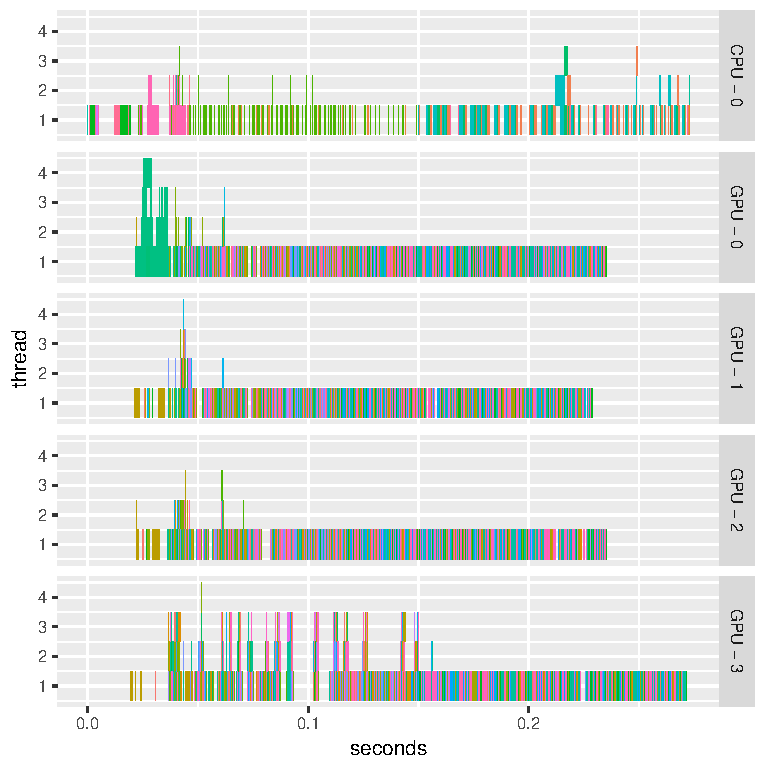
\includegraphics[width=\textwidth]{bytenet/profile-raw-gpu4.pdf}
    \caption{Shows time spend on each operation, when the operation was executed, and on what GPU/CPU it was executed. The color coding indicates the operation type, there are more than a 100 different operation types, most are specific to TensorFlow, thus the legend is not included.}
    \label{fig:result:bytenet:profile-raw}
\end{figure}

To understand why the ByteNet model is so slow, TensorFlow was profiled while executing the computational graph. The setup is identical to the ``Memorizing WMT NewsTest'' setup running on 4 GPUs, and the profiling was done when evaluating the 4500th mini-batch. The 4500th mini-batch was chosen because the performance has reached its peak and stabilized.

From figure \ref{fig:result:bytenet:profile-raw} it's seen that most of the time is not spend computing, but rather waiting for data to be transferred or just waiting for the TensorFlow service to queue a new task.

\begin{figure}[h]
    \centering
    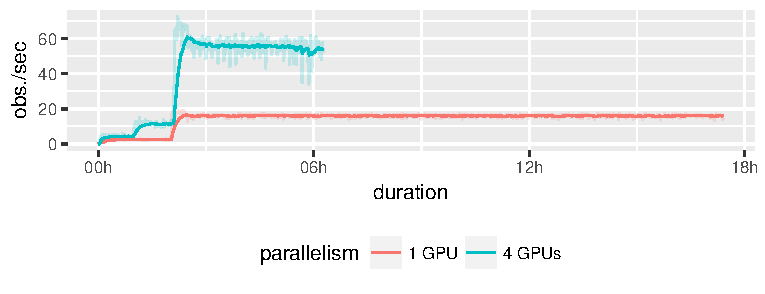
\includegraphics[scale=1]{bytenet/timing-gpus.pdf}
    \caption{Comparing observations per second, depending on the number of GPUs used.}
    \label{fig:result:bytenet:timing-gpus}
\end{figure}

By comparing the speed of how fast the ByteNet implementation processes observations, depending on the number of GPUs used, one gets that about 37\% of the time is spent waiting for data transference in the 4 GPUs case. This calculation does, in particular, make sense when comparing with 1 GPU, since a 1 GPU setup will not require data transfer of any weights. This is because the gradients and weights don't need to be synchronized on the CPU, but can be kept on the GPU where they are calculated.

The data transfer does not explain all the waiting time. Likely this particular profiling is an extreme case. TensorFlow transfers the dataset in chunks in preparation for future mini-batches. If TensorFlow is transferring the dataset while profiling in this exact moment, that will cause extra waiting time.

By processing the profiling dump file, such that the waiting time is removed from the data, one can see that time is primarily spent in the layers that contain normalization and activation (\textit{pre-normalization}, \textit{conv-dilated}, \textit{reduce-dim}).

\begin{figure}[h]
    \centering
    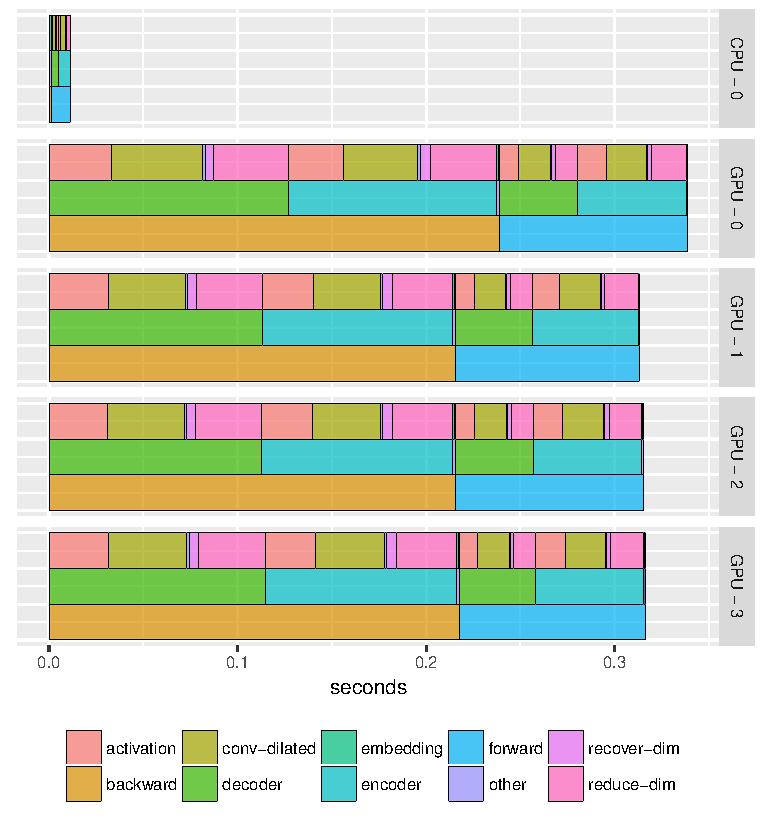
\includegraphics[scale=1]{bytenet/profile-grouped-gpu4.pdf}
    \caption{Shows time spend executing each part of the ByteNet model, this excludes the waiting time. Each part exists in a hierarchy, which is visualized as levels. Bottom level is the backward and forward pass. Second level is the encoder and decoder. Last level primarily splits the ByteNet Residual Blocks.}
    \label{fig:result:bytenet:profile-grouped}
\end{figure}

It is likely that the data transfer part could be optimized, but in general, this isn't easy and there are practical limitations to how much it can be improved. It is much more likely that the waiting time regarding the TensorFlow service could be improved.

TensorFlow works with a computational graph. Each atomic operation, like an element-wise addition or a matrix multiplication, is a node in this graph and the edges describe the dependencies. The TensorFlow service will watch the graph and execute any node (atomic operation) when all its dependencies are satisfied, it will even execute multiple nodes in parallel if possible. This process repeats until all nodes have been computed and the end result is obtained.

Using a computational graph is a good strategy, but the current TensorFlow implementation of it is very naive. TensorFlow uses no-op and identity operations, which only exists because of TensorFlow semantics, but don't need to be executed. However, in the current state of TensorFlow, it just executes all nodes naively. There are also numerous of atomic operations that could be fused into one atomic operation. An example is batch normalization that involves quite a few element-wise operations, all these are executed separately but could be combined into a single atomic operator. All these atomic operators are what causes the waiting time, the TensorFlow service needs to walk the computational graph and more importantly just launching GPU kernels also introduces wasted time.

The TensorFlow team is aware of the current limitations and are in the process of solving these issues, by using a Just In Time compiler that can automatically fuse many of these operations. But so far this is in an experimental state and performs very poorly when running on multiple GPUs \cite{google-xla}.
